
\section{Implementation}
\label{sec:impl}

\subsection{Overview}

\paragraph{System Architecture}

\begin{figure}
\begin{centering}
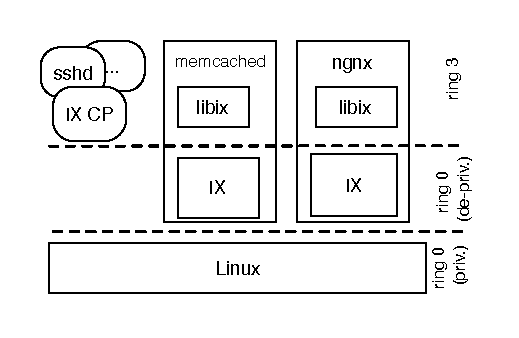
\includegraphics{figs/cp-dp.eps}
\centering\caption{Protection and separation in \ix.}
\label{fig:cp-dp}
\end{centering}
\end{figure}



\paragraph{Protection using hardware virtualization}


\paragraph{Multi-Queue and Bonding}

\begin{figure}
\hspace*{-0.25in}\centering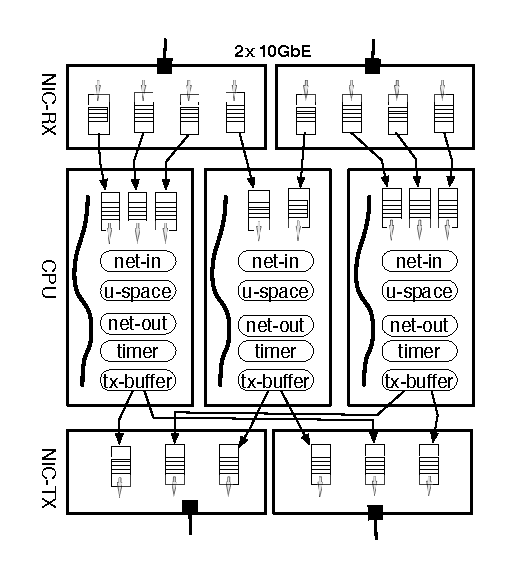
\includegraphics{figs/queues-cores.eps}
\caption{Example of IX scaling across two NICs interfaces, 8 NIC RX queues, and 3 CPU hardware threads.} 
\label{fig:queues-cores}
\end{figure}


%\begin{figure}
\begin{centering}
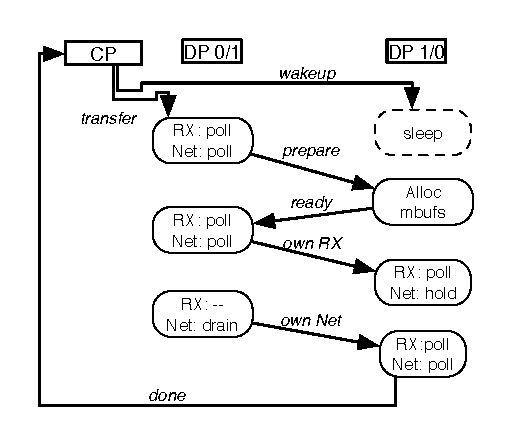
\includegraphics{figs/queue-takeover.eps}
\caption{Queue takeover algorithm.}
\label{fig:queue-takeover}
\end{centering}
\end{figure}




\paragraph{Resource allocation}


\subsection{The \ix Pipeline}

\begin{figure}
\begin{centering}
% FIXME
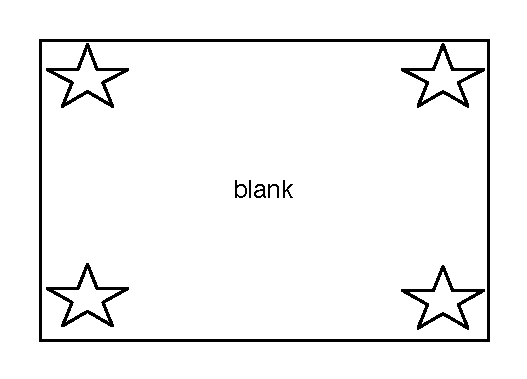
\includegraphics{figs/blank.eps}
\caption{Main stages of the \ix pipeline.}
\label{fig:pipeline}
\end{centering}
\end{figure}



\todo   Fig.~\ref{fig:mainloop} state machine (main loop)
\todo   batching, stage, main loop, ...
\todo   hardware optimization
\todo   the driver layer
\todo   TCP processing
     
\subsection{The \ix native API}

\begin{figure}
\begin{centering}
% FIXME
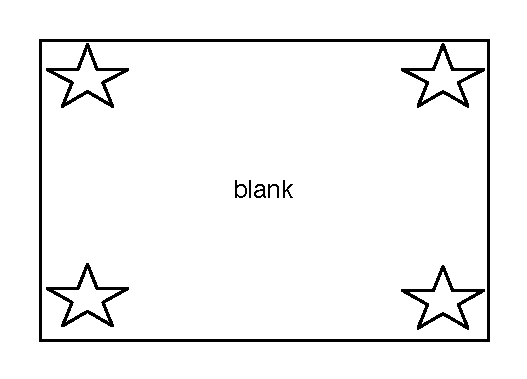
\includegraphics{figs/blank.eps}
\caption{Zero-copy, event-driven ping-pong server using the native \ix API.}
\label{fig:listing}
\end{centering}
\end{figure}


\todo Fig.~\ref{fig:listing} Listing .. (echo server)
\todo list of events (is it like Megapipe and/or mTCP)
\todo  true zero-copy

\subsection{LibEvent Compatibility}

\todo Details 

\christos{if we can sqeeze in an app example (pseudocode for echo
  server) it would be great}

\subsection{Congestion management and flow control}

\todo memory maangement
\todo secure application flow control
\todo congestion detection
\todo congestion notification

\subsection{Discussion}

\todo any loose ends

\todo explicitly list future work (more complete TCP, policies for elasticity)


